\documentclass[]{elsarticle} %review=doublespace preprint=single 5p=2 column
%%% Begin My package additions %%%%%%%%%%%%%%%%%%%

\usepackage[hyphens]{url}


\usepackage{graphicx}
%%%%%%%%%%%%%%%% end my additions to header

\usepackage[T1]{fontenc}
\usepackage{lmodern}
\usepackage{amssymb,amsmath}
% TODO: Currently lineno needs to be loaded after amsmath because of conflict
% https://github.com/latex-lineno/lineno/issues/5
\usepackage{lineno} % add
\usepackage{ifxetex,ifluatex}
\usepackage{fixltx2e} % provides \textsubscript
% use upquote if available, for straight quotes in verbatim environments
\IfFileExists{upquote.sty}{\usepackage{upquote}}{}
\ifnum 0\ifxetex 1\fi\ifluatex 1\fi=0 % if pdftex
  \usepackage[utf8]{inputenc}
\else % if luatex or xelatex
  \usepackage{fontspec}
  \ifxetex
    \usepackage{xltxtra,xunicode}
  \fi
  \defaultfontfeatures{Mapping=tex-text,Scale=MatchLowercase}
  \newcommand{\euro}{€}
\fi
% use microtype if available
\IfFileExists{microtype.sty}{\usepackage{microtype}}{}
\usepackage[]{natbib}
\bibliographystyle{plainnat}

\ifxetex
  \usepackage[setpagesize=false, % page size defined by xetex
              unicode=false, % unicode breaks when used with xetex
              xetex]{hyperref}
\else
  \usepackage[unicode=true]{hyperref}
\fi
\hypersetup{breaklinks=true,
            bookmarks=true,
            pdfauthor={},
            pdftitle={Title here},
            colorlinks=false,
            urlcolor=blue,
            linkcolor=magenta,
            pdfborder={0 0 0}}

\setcounter{secnumdepth}{0}
% Pandoc toggle for numbering sections (defaults to be off)
\setcounter{secnumdepth}{0}


% tightlist command for lists without linebreak
\providecommand{\tightlist}{%
  \setlength{\itemsep}{0pt}\setlength{\parskip}{0pt}}







\begin{document}


\begin{frontmatter}

  \title{Title here}
      \cortext[cor1]{Corresponding author}
  
  \begin{abstract}
  The text of your abstract. 150 -- 250 words.
  \end{abstract}
    \begin{keyword}
    key \sep dictionary \sep 
    word
  \end{keyword}
  
 \end{frontmatter}

\hypertarget{introduction}{%
\section{Introduction}\label{introduction}}

In education, there's interest in identifying reliable indicators for
teacher stress and burnout {[}\citet{fisher2011}; @ junker2021{]}.
Previous research often relied on self-report questionnaires
\citep{chaplain2008, liu2020}, which may be prone to biases like social
desirability \citep{razavi2001self} or recall errors
\citep{van2016accuracy}. To overcome these limitations, ambulatory
assessment methods are recommended
\citep{trull2013ambulatory, wettstein2020ambulatory}, such as measuring
physiological parameters like heart rate (HR), offering objective
insights into teachers' stress levels without disrupting their teaching
\citep{donker2018, runge2020}.

Current studies on teachers' HR in teaching settings often rely on
expensive and invasive electrocardiographs
\citep{sperka1995, scheuch1997psychophysische, donker2018, junker2021, huang2022class},
showing that teacher-centered activities and common stressors lead to
increased HR. However, using affordable and non-invasive instruments
like wrist-worn fitness trackers \citep{ferguson2015} could enhance HR
recording in educational contexts. Unlike clinical devices, fitness
trackers could offer continuous and less intrusive data collection over
time \citep{godfrey2018z}, aligning with the increasing popularity and
acceptance of wearables among the general population
\citep{peng2022acceptance}. These devices, equipped with biosensors,
provide users with physiological and behavioral data, offering an
accessible means for monitoring physical activity and health in daily
life.

It can be assumed that teachers also wear personal, private fitness
trackers, generating recordings of physiological data that could be a
very interesting resource for research on teacher stress. While the use
of wearable technology in the field has been explored in various domains
{[}\citet{hughes2023wearable}; @ adesida2019exploring;
helmer2009smart{]}, research is sparse in educational contexts
\citep{de2017towards}. Although some studies investigated how wearables
can help teachers monitor student activity \citep{quintana2016keeping},
there is a notable research gap regarding teachers' use of wrist-worn
wearables. Given the high stress levels in the teaching profession
\citep{johnson2005experience}, fitness trackers could be a valuable tool
for analyzing HR and the factors contributing to stress. One of the
reasons for teachers' augmented stress is that they are confronted with
a multitude of demands in their everyday work, some of which exceed
their resources and therefore make it difficult to cope with immediate
stressors such as classroom disruptions \citep{montgomery2005meta}.
However, the extent of the strain depends on the subjective appraisal of
a stressor, which involves considerations about available resources to
deal with it \citep{kyriacou2001}. It is, therefore, particularly
important for teachers to have sufficient personal and professional
resources at their disposal \citep{cramer2018belastung}. Classroom
disruptions, for example, are one of the major stressors in teachers'
daily work \citep{boyle1995structural, aloe2014multivariate} and
professional knowledge about effective classroom management reduces the
risk of teacher stress \citep{klusmann2012berufliche}. Teachers'
characteristics such as professional experience in turn have an impact
on the development of classroom management skills and thus on the
appraisal processes, as these skills develop during professional
experience \citep{ophardt2017klassenmanagement, wolff2015keeping}.

To better understand how stressors like classroom disruptions affect
teachers and their stress responses, data from wrist-worn fitness
trackers could be used to monitor physiological parameters before,
during, and after teaching sessions \citep{wettstein2021}. This study
explored the use of wrist-based fitness trackers as a tool to monitor
teachers' stress during different phases of a micro-teaching unit during
which teachers had to deal with classroom disruptions. Physiological
data were triangulated with teachers' appraisal of classroom
disruptions, and their teaching experience. The physiological indicator
employed in this study was teachers' HR, which can be readily recorded
by any fitness tracker. Teachers' use of wrist-worn fitness trackers in
educational research holds transformative potential as obtained
fine-grained data and underscores the critical need to monitor teachers'
health as they navigate the stressful landscape of the classroom.

\hypertarget{fitness-trackers-as-a-method-to-assess-hr-as-an-indicator-of-stress}{%
\subsection{Fitness Trackers as a Method to Assess HR as an Indicator of
Stress}\label{fitness-trackers-as-a-method-to-assess-hr-as-an-indicator-of-stress}}

Wearables, defined as electronic devices worn directly on the body or
integrated into clothing or accessories, serve as versatile solutions
\citep{godfrey2018z}, gathering data like location, movements, and vital
signs \citep{cheng2017underlying}. Fitness trackers, a popular wearable
type \citep{park2020user}, offer insights into physical activity and
cardiovascular health, supporting personalized fitness goals
\citep{nuss2021effects} and stress management \citep{hao2018chrv}. Their
affordability and ease of use make them ideal not only for various
domains including healthcare, entertainment, and fitness
{[}sinha2019taxonomy{]} but also in education as they offer added
benefits for formal and informal learning environments for both students
and teachers \citep{de2017towards}. Yet, few studies focus on their
significance for teachers.

One important health parameter assessed by nearly all wrist wearables is
HR \citep{scalise2018wearables}. HR indicates the number of heartbeats
within one minute and is typically expressed as beats per minute (BPM)
\citep{hottenrott2007}. At rest, the average HR of adults typically
ranges from 60 to 80 BPM \citep{sammito2015guideline}. HR can be
detected and measured using sensors based on electrocardiogram (ECG) or
phonocardiogram (PCG) \citep{mukhopadhyay2017wearable}. Another
uncomplicated and inexpensive technique to measure HR via fitness
trackers is photoplethysmography (PPG) \citep{castaneda2018review}. This
optical method assesses HR by flashing green or red lights to measure
changes in blood volume \citep{allen2007photoplethysmography}.\\
Physiologically, HR is regulated and influenced on short-time intervals
by the sympathetic and the parasympathetic nervous system
\citep{pham2021}. An increase in the activity of the sympathetic system
results in HR being speeded up (``fight or flight'')
\citep{taelman2009influence}. In contrast, increased activity of the
parasympathetic has the effect of slowing down the HR (``rest and
digest'') \citep{battipaglia2015}. Therefore, an increase in HR can be
regarded as an indicator of increasing stress, and a decrease as an
indicator of decreasing stress \citep{kyriacou1978}.

\hypertarget{teacher-stress-and-important-resources}{%
\subsection{Teacher Stress and Important
Resources}\label{teacher-stress-and-important-resources}}

The teaching profession is one of the most stressful professions
compared to other occupational groups, facing a variety of stressors
during everyday work \citep{smith2000, herman2020, schult2014belastet}.
According to \citet{kyriacou1978}, teacher stress can be defined as a
negative affective response, often accompanied by physiological changes
such as increased HR, triggered by job-related demands and perceived as
threatening to one's self-esteem or well-being. Coping mechanisms help
to reduce the perceived threat.

This definition of teacher stress is based on the transactional stress
model by Lazarus and colleagues
\citep{lazarus1981stressbezogene, lazarus1984stress}, which was modified
and tailored to the teaching-learning environment by
\citet{kyriacou1978}.

In general, the transactional stress model \citep{lazarus1990theory}
highlights the interaction between an individual and the environment,
whereby stress refers to any event that exceeds a person's adaptive
resources. It has been shown that there are important connections
between stressors and resources experienced by teachers on the one hand,
and stress-induced health issues on the other hand
\citep{krause2013messung}. As we are interested in how specific
classroom events affect teacher stress, we adapted the transactional
stress model to that type of situation, based on a representation of the
model first proposed by {[}van2006stress{]}; this working model is
depicted in Fig. 1.

\begin{figure}[htbp]
  \centering
  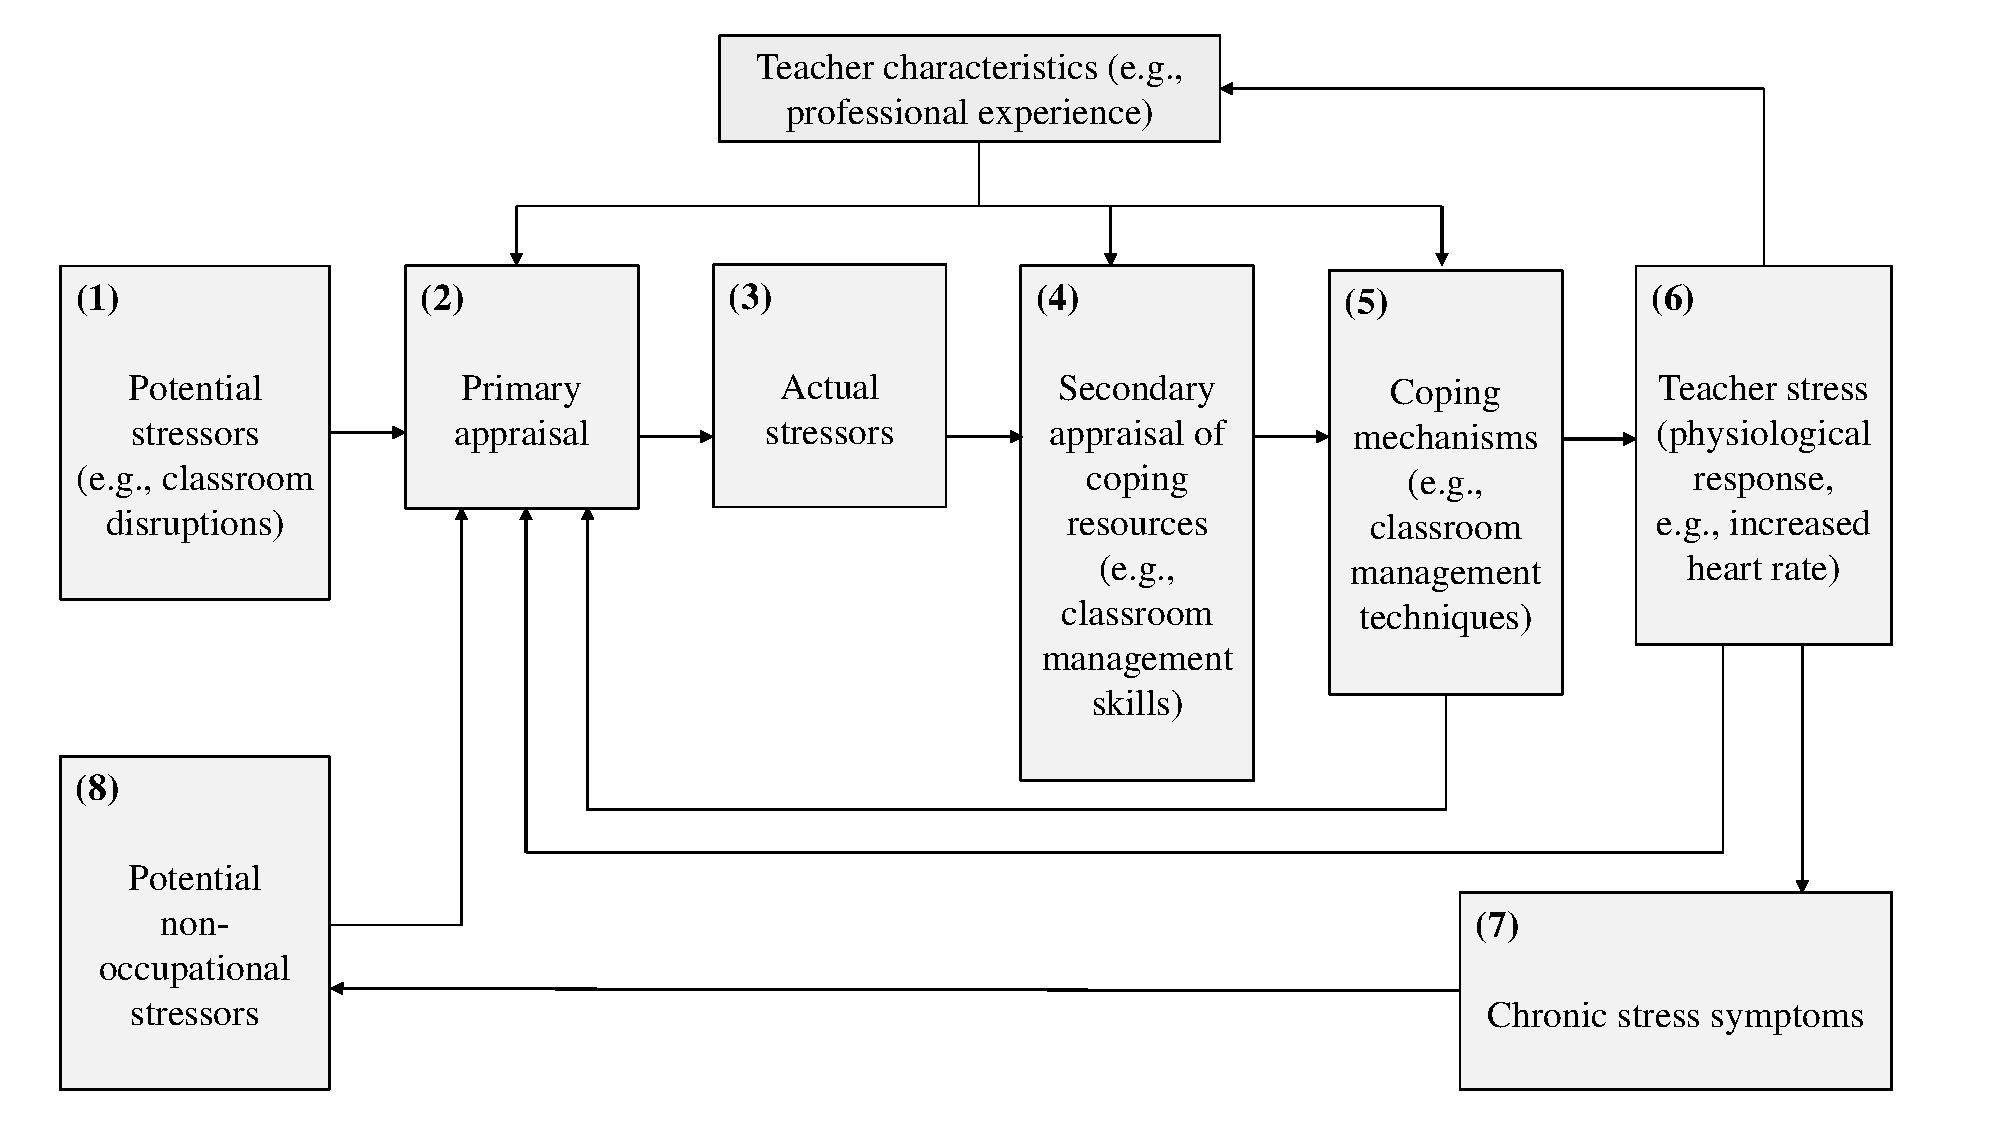
\includegraphics[width=1\textwidth]{images/Model_Teacher_Stress_adapted_new.pdf}
  \caption{A model of teacher stress (adapted from van Dick 2006, p.37, modified by the author)}
  \label{A model of teacher stress (adapted from van Dick 2006, p.37, modified by the author)}
\end{figure}

When potential stressors (e.g., classroom disruptions) occur during
teaching (1), teachers subjectively appraise how disruptive the event is
(2). If potential stressors are judged as threatening, i.e., as actual
stressors (3), teachers consider whether they have sufficient resources
for coping with the stressor (4). Based on this evaluation of resources
and their characteristics such as professional experience, teachers try
to manage classroom disruptions, by utilizing classroom management
strategies (5). In cases where coping fails, stress ensues, often
accompanied by physiological reactions like increased HR (6). Following
resource appraisal and coping outcomes, the stressor is re-evaluated
(7).

The appraisal processes of resources play a crucial role as teachers'
assessments of resources and coping mechanisms, both internal (e.g.,
classroom management skills) and external (e.g., supportive colleagues),
significantly impact their stress levels. When resources are lacking and
coping fails, negative consequences like burnout and high turnover can
arise \citep{jalongo2006, unterbrink2007, aloe2014}. This highlights the
importance of teachers' appraisal of their professional competencies,
including their ability to manage classroom disruptions effectively
\citep{klieme2008concept, konig2016teacher}.

As shown in Fig. 1, both primary and secondary appraisals are influenced
by teachers' characteristics, e.g., their professional experience,
shaping their classroom management skills. As experience grows, teachers
develop cognitive scripts for managing classroom events resulting in
more complex classroom management skills \citep{wolff2021classroom}.
Especially beginning teachers face considerable stress and often feel
overwhelmed by the demands of teaching
{[}\citet{ophardt2017klassenmanagement}; \citet{wolff2015keeping}; @
klusmann2012berufliche{]}, with many leaving the profession within the
first five years \citep{ingersoll2003}. Research shows less experienced
teachers are more susceptible to burnout, underscoring the importance of
experience and job satisfaction in predicting teacher stress
\citep{fisher2011}.

\hypertarget{hr-in-teaching-learning-contexts}{%
\subsection{HR in Teaching-Learning
Contexts}\label{hr-in-teaching-learning-contexts}}

ECG studies have revealed that HR can be used to map changes in HR
during teaching onto stressors experienced by teachers. For example, HR
increased during teacher-centered activities when teachers had to take a
leading position in the student-teacher interaction
\citep{sperka1995, scheuch1997psychophysische, donker2018, junker2021}.
\citet{sperka1995} for example recorded the HR of 16 pre-service
teachers during their first lesson. The results showed significantly
increased psychophysiological activation in terms of an increased HR
during teaching. The activation effect was particularly prominent at the
beginning of the lesson and decreased over the course of the lesson. The
authors interpret this result as showing how pre-service teachers'
active coping processes, i.e., the active management of the interaction
with the students, helped the teachers regulate their HR downwards.
Other ECG studies identified typical stressors predicting increased HR
values, such as class size \citep{huang2022class}, or low student
engagement and motivation \citep{junker2021}. For example,
\citet{junker2021} recorded the HR of 40 teachers using an ambulatory
monitoring system during a real classroom lesson. They provided evidence
that teacher stress caused by stressors such as low student engagement,
i.e., students displaying a lack of motivation or limited interest in
their tasks or classroom activities, or teacher-centered activities,
i.e., classroom activities primarily focused on the teacher's actions.,
leads to an increase in HR.

In addition to ECG studies, there are a few studies that used wrist-worn
fitness trackers to investigate HR trends in teaching-learning
situations \citep{Darnell2019, chalmers2021}. \citet{Darnell2019} for
example measured the HR of 15 medical college students using wrist-worn
devices during lectures. The analysis revealed a constant decrease in HR
from the beginning to the end of a lecture, whereas the HR peak was
reached during active learning sessions. \citet{chalmers2021} examined
the usability of the average HR, measured with a Fitbit fitness tracker,
to identify physiological changes during stress-inducing tasks in a
study with a total of 60 participants. The average HR increased
significantly between the resting and stress phases. Even though the
participants in these studies were learners, not teachers, the results
are relevant to the study of teacher stress using wearable devices,
because the studies showed that a) HR can be effectively recorded using
fitness trackers during a whole learning unit, and b) HR changes are in
line with the occurrence of activating or stress-inducing tasks.

So far, to the best of our knowledge, only one study has directly
assessed teachers' HR using a wrist-worn fitness tracker during teaching
: \citet{runge2020} used a Fitbit fitness tracker to assess HR as an
indicator of stress in N=4 teachers. They used the fitness trackers'
recordings to create a profile for each teacher (to differentiate
between teachers reporting higher or lower levels of stress .) In
particular, it was found that the combination of a high number of steps,
a high HR, and short sleep was an indicator of stress. It should be
noted that the generalizability of the results is limited due to the
small sample size.

In summary, previous studies have revealed that teachers' (and
students') HR changes, depending on the activity and stressors they
experience, whereby teacher-centered phases , in particular, led to an
increase in HR
\citep{sperka1995, scheuch1997psychophysische, donker2018, junker2021}.
Furthermore, it could be shown that HR as an indicator of stress can be
assessed using low-cost, non-intrusive fitness trackers and that HR
increases in activating phases and even before stress occurs
\citep{Darnell2019, chalmers2021}. However, studies collecting data from
teacher-worn fitness trackers in a large enough sample to explore links
with factors such as subjective stressor appraisal, or effects of
teaching experience, are still lacking. Our study aims to close this
research gap.

\hypertarget{present-study}{%
\subsection{Present Study}\label{present-study}}

The data analyzed for the present study were obtained from teachers and
student teachers who participated in a lab study, as part of a larger
project targeting the development of classroom management in teachers.

As part of the larger project, participants came to the lab
individually, and each taught a 15-minute, self-prepared micro-teaching
unit to a ``class'' of three actors (trained student assistants). These
actors performed nine, possibly disruptive, classroom events. The actors
received standardized instructions on a screen (only visible to them,
not to the participant) to perform a classroom event every one and a
half minutes, and they performed the same scripted disruptions for all
participants. While teaching, participants wore eye-tracking glasses,
and additionally, their lessons were recorded by cameras.

The micro-teaching unit, with its unfamiliar setting and the scripted
disruptions of participants' teaching flow, was potentially stressful.
Thus, we were particularly interested in the development of
participants' HR before, during, and after this micro-teaching unit. We
recorded HR data in five phases, with a total duration of approximately
two hours: In the \emph{pre-teaching phase}, participants were welcomed,
prepared for the following micro-teaching unit, and familiarized with
the setting. In the \emph{teaching phase}, participants taught the
micro-teaching unit and experienced the classroom disruptions. In the
\emph{post-teaching phase}, participants answered several questionnaires
in a comfortable seated position. Next, in the \emph{interview phase},
they watched the video of their 15-minute unit, rated the disruptive
classroom events, and answered open questions. Finally, in the \emph{end
phase}, participants answered another questionnaire. These conditions
were identical for all participants. During the entire study,
participants wore a fitness tracker on their wrist.

The goals of the present study were twofold:

\begin{enumerate}
\def\labelenumi{(\arabic{enumi})}
\tightlist
\item
  The first research goal was to investigate whether HR measures
  assessed by wrist-based fitness trackers are a suitable and effective
  method for mapping teachers' HR over the course of a five-phase lab
  study, including the time before, during, and after a potentially
  stressful micro-teaching unit.
\end{enumerate}

First, we expected the participants to show an initial increase in their
HR, followed by a peak during the teaching phase and a decrease for the
remaining phases. In addition, we examined whether z-standardization of
the participants' mean HR could serve as a useful method to account for
individual differences in baseline HR. We expected to observe the same
trends in both standardized and non-standardized mean HR values.

Second, five representative 10-minute intervals were selected from the
five phases (see section \#\#Measures for a more detailed description of
the intervals), which served as the basis for the data analysis for our
hypothesis: pre-teaching interval (\(I_1\)), teaching interval
(\(I_2\)), post-teaching interval (\(I_3\)), interview interval
(\(I_4\)), end interval (\(I_5\)). We examined the levels of and the
changes in HR during these intervals. We assumed the highest HR level in
the teaching interval (\(I_2\)) and lower levels in all other intervals
(\textbf{Hypothesis 1a}). Further, we expected an increase in
participants' HR while they were preparing for teaching during the
pre-teaching interval (\(I_1\)), and we expected a decrease in
participants' HR during all of the following intervals, because of
habituating to (\(I_2\)) and recovering from (\(I_3\)-\(I_5\)) the
stressful teaching phase (\textbf{Hypothesis 1b}).

\begin{enumerate}
\def\labelenumi{(\arabic{enumi})}
\setcounter{enumi}{1}
\tightlist
\item
  The second research goal was to examine whether variance in HR
  measures could be explained by participants' teaching experience
  (because, presumable, more experienced teachers might have better
  classroom management strategies, and thus better resources for
  coping), and/or by their self-reported subjective appraisals of
  classroom events (specifically, how disruptive it was, and how
  confident they felt in their coping).
\end{enumerate}

We expected lower HR levels for teachers with more teaching experience,
particularly during the teaching interval (\textbf{Hypothesis 2a}). We
expected higher HR levels for teachers who felt more disrupted by the
enacted classroom events, regardless of their teaching experience
(\textbf{Hypotheses 2b}). At the same time, we expected lower HR levels
for teachers who felt more confident in dealing with the events,
regardless of teaching experience (\textbf{Hypothesis 2c}). Lastly, we
hypothesized that each of the three predictors (teaching experience,
disruption appraisal, confidence appraisal) uniquely contributes to
explaining variance in teachers´ HR levels (\textbf{Hypothesis 2d}). In
addition, we exploratively examined the same as for the HR levels again
for the changes in HR.

\hypertarget{method}{%
\section{Method}\label{method}}

\hypertarget{participants}{%
\subsection{Participants}\label{participants}}

The sample consisted of \(N\) = 84 pre- and in-service teachers from
Germany, who were recruited via personal contact, email lists, and
flyers. The data of three participants was lost due to failed data
transmission, yielding an analysis sample of \(n\) = 81 (\(n\) = 52
women, \(n\) = 29 men). Participants had a mean age of 30.95 years
(\(SD\) = 10.90; range: 19-60) and an average teaching experience of
5.64 years (\(SD\) = 9.46; range: 0-37).

\hypertarget{setting-and-procedure}{%
\subsection{Setting and Procedure}\label{setting-and-procedure}}

The study was carried out following the ethical standards and the
approval of the University's Institutional Review Board. All
participants were informed in detail about the aims and intention of the
study before testing. Participation was voluntary and only took place
after written consent had been given. Participants were not rewarded in
any way for participating in the study.

\begin{figure}[htbp]
  \centering
  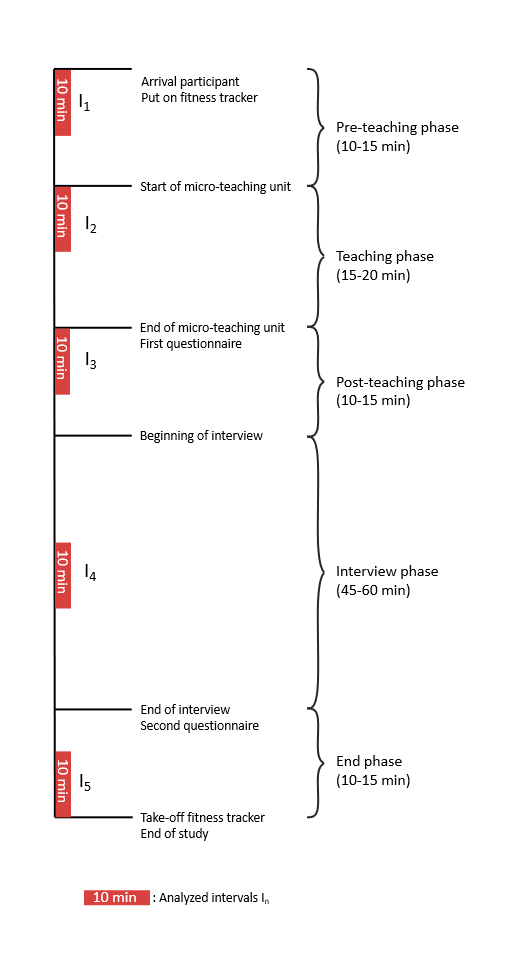
\includegraphics[width=1\textwidth]{images/Timeline_ProVision_vertical.png}
  \caption{Procedure of the two-hour-long study consisting of five phases with five representative 10-minute intervals}
  \label{Procedure of the two-hour-long study consisting of five phases with five representative 10-minute intervals}
\end{figure}

Each participant came to the lab for a period of approximately two hours
in total, and each underwent the same phases: \emph{pre-teaching phase},
\emph{teaching phase}, \emph{post-teaching phase}, \emph{interview
phase}, and \emph{end phase} (please refer to Fig. 2 for a timeline). In
the \emph{pre-teaching phase}, the experimenter welcomed the
participants and helped them put on the fitness tracker. This was
followed by a warm-up session to familiarize the participants with the
laboratory setting and the class. This phase took about 10-15 minutes
and participants spent this time mostly standing or slowly walking
around. During the \emph{teaching phase}, the participants held their
self-prepared, micro-teaching unit to a class of three trained actors
who performed nine, potentially disruptive, classroom events (e.g.,
chatting with a neighbor, heckling, looking at the phone; see Table \#\#
in the supplementary material for an overview and categorization of all
events; also see Fig\#\# for a depiction of the laboratory setting of
the micro-teaching unit). In preparation for the 15-minute lesson, the
topic and class level could be freely chosen by the teachers. The type
of course was to be an introductory lesson and the desired social form
required individual work or frontal teaching, without longer video
sequences and movement of the actors. The teaching unit lasted about
15-20 minutes. Participants spent this time mostly standing or slowly
walking around. After having completed the micro-teaching unit, in the
\emph{post-teaching phase}, participants were seated at a desk and
filled in questionnaires for approximately 10-15 minutes: a brief
computer-based questionnaire assessing sociodemographic data (e.g.,
teaching experience, gender, studied school type, studied school
subjects, extracurricular teaching activities), and a short knowledge
test that is irrelevant to the present study. In the \emph{interview
phase}, the participants watched the video of their own teaching
together with the experimenter. While doing so, they were given a
Stimulated Recall Interview (SRI), in which the participants watched
their recorded eye-tracking video of the lesson from the ego
perspective, indicating the participants' gaze point. The experimenter
stopped the video each time one of the nine classroom events happened
and asked a total of eight questions, five of which were open and three
closed. We assessed -- among other questions irrelevant to this study --
with two closed questions the teachers' subjective appraisal of the
classroom events that took place during the \emph{teaching phase} in
terms of how subjectively disruptive they were (disruption appraisal)
and how confident the participants felt dealing with them (confidence
appraisal) with one item each. The interview lasted about 45-60 minutes
and the participants' position was seated. The \emph{end phase} lasted
about 10-15 minutes and participants answered in a seated position
another questionnaire irrelevant to this study.

\hypertarget{measures}{%
\subsection{Measures}\label{measures}}

\hypertarget{heart-rate-data-and-heart-rate-intervals}{%
\subsubsection{Heart Rate Data and Heart Rate
Intervals}\label{heart-rate-data-and-heart-rate-intervals}}

To measure the teachers' HR, we used a wrist-based fitness tracker. The
model was a Fitbit Charge 4. In line with the manufacturer's
instructions \citep{fitbitnd}, the device was attached a finger's width
above the participants' nondominant hand's wrist bone. The tracker works
by flashing green LEDs hundreds of times per second, using
light-sensitive photodiodes to catch the reflected light, and from that
information calculating volume changes in the capillaries. From this,
the tracker calculates how many times the heart beats per minute. HR
measurements are generated at least every 15 seconds\footnote{The
  fluctuations in the number of seconds in which the HR was measured are
  due to the participants' movements, meaning that the device could not
  measure the HR every second.}. The raw data that can be extracted from
the tracker lists the time stamps of all measurements and the estimated
HR in BPM for each time stamp.

The anonymous HR data was synced via Bluetooth to a commercial Fitbit
account. Subsequently, the intraday second-by-second data was exported
as a CSV file for each session using the open-source software PulseWatch
(Ricci, n.d.), and linked to the participant. To account for individual
differences in the baseline HR, we first z-standardized the BPM values
from the unstandardized mean HRs.

Since we aimed to explore teachers' HR between different strain phases,
we aggregated HR over a 10-minute interval within each phase. Previous
research has indicated that 10-minute intervals are a useful duration
for analyzing PPG data \citep{lu2008can}. The intervals were selected
based on the following rules: The pre-teaching interval (\(I_1\))
comprised the first 10 minutes after the fitness tracker had been put
on. The teaching interval (\(I_2\)) started two minutes after the
teacher had started the teaching unit. This interval was of the highest
relevance to our study. We explicitly chose an early 10-minute interval
within the teaching phase, as previous studies revealed that the
beginning of a lesson is essential and demanding regarding
teacher-student interaction
\citep{donker2018quantitative, claessens2017positive}. The post-teaching
interval (\(I_3\)) started immediately after the end of the teaching
unit. The interview interval (\(I_4\)) was defined as the mid-10 minutes
between the end of the teaching unit and the time point when the fitness
tracker was taken off so that all participants were being interviewed
during this interval. The end interval (\(I_5\)) comprised the last 10
minutes before the fitness tracker was taken off.

\hypertarget{teaching-experience}{%
\subsubsection{Teaching Experience}\label{teaching-experience}}

The participants' teaching experience was assessed as a part of
sociodemographic data. Participants stated their work experience in
years (excluding the traineeship year).

\hypertarget{subjective-appraisal-of-the-classroom-events-and-coping-processes}{%
\subsubsection{Subjective appraisal of the classroom events and coping
processes}\label{subjective-appraisal-of-the-classroom-events-and-coping-processes}}

The subjective disruption and confidence appraisals assessed in the SRI
on an 11-point rating scale were averaged across the nine classroom
events as we were not interested in individual classroom events, but
only in the expected mean level of arousal during the \emph{teaching
phase}. Regarding the model (see Fig. 1), the disruption appraisal was
used to assess the evaluation of the stressor (see Fig. 1, box 2). The
confidence appraisal, in contrast, referred to the resources available
for coping with the stressors (see Fig. 1, box 4).

\hypertarget{data-analysis}{%
\subsection{Data analysis}\label{data-analysis}}

We conducted all analyses with R \citep{RStudio2020}. Graphics were
created using ggplot2 (v3.3.3; Wickham, 2016).

\textbf{Research goal 1}. The first research goal included mapping
teachers' HR before, during, and following a micro-teaching unit in the
course of a five-phase lab study.

Regarding the teachers' HR trend, we displayed the HR trend over the
course of the entire study. For z-standardization as a method to account
for individual differences in the baseline HR, we visually compared
unstandardized and standardized mean HR trends for the entire two-hours
study. For testing Hypothesis 1a, which examined the HR levels in the
different intervals, we initially conducted a one-way ANOVA with
repeated measures as an omnibus test. The dependent variable comprised
the standardized HR mean for each interval. To identify the highest HR
level, we subsequently conducted t-tests with planned contrasts as
post-hoc tests, accompanied by the effect size d \citep{cohen1988new}.
Specifically, we tested the differences between the teaching interval
(\(I_2\)) and the other four intervals. Note that mean HR was calculated
at the subject level of \(n\) = 81 participants (see Table 1), whereas
the mean slope and mean intercept estimates are based on all values at
all measurement time points (see Table 2). For testing Hypothesis 1b,
which examined the HR changes within each interval, we conducted a
linear estimation of the increase or decrease in HR over time. To this
end, we used fixed intercept fixed slope regression models
\citep{gelman2006data} for each interval to estimate intercepts and
linear slopes for all individuals which were then averaged across
individuals\footnote{Although this procedure does not account for
  nonmonotonic progressions in individual HR, a graphical evaluation
  revealed that the linear estimates corresponded well to the majority
  of the cases (see XX in the supplementary material).}.

\textbf{Research goal 2}. In addressing our second research goal, we
examined the effects of teaching experience and subjective appraisal of
disruptive classroom events on teachers' HR levels during the five
phases.

To test hypothesis 2a, we examined the effect of teaching experience on
participants' HR levels for each of the five intervals using linear
regression models with teaching experience as the sole predictor. To
test hypotheses 2b and 2c, we separately augmented the models by either
teachers' disruption appraisal (Hypothesis 2b) or confidence appraisal
(Hypothesis 2c), while controlling for shared variance with teaching
experience. HR levels were only predicted with the disruption and
confidence appraisal after the teaching had taken place, i.e., for all
the intervals following the pre-teaching interval (I1). To test
hypothesis 2d, we examined the effects of all three predictors in one
regression model. We repeated these steps to explore the effect of
teaching experience and subjective appraisals on changes in teachers' HR
at each interval.

\bibliography{r-references.bib}


\end{document}
